\documentclass{article}

\usepackage{algorithm}
\usepackage{algpseudocode}
\usepackage{graphicx}
\usepackage{subcaption}

\title{AIML426 Project 2 Report}
\date{}

\begin{document}
	\maketitle
	
\section*{Part 1: Evolutionary Programming and Differential Evolution Algorithms}
\subsubsection*{Individual Representation}
An individual solution is represented as a sequence of D float values that are used for the variables to be applied to the function used for the fitness function. Each element in the sequence is associated with one variable to be used. D represents the number of variables used by the fitness function. \par
\subsubsection*{Fitness Function}
The fitness function is the value produced by the function with the variable values stored in the individual. The function used is either Rosenbrock or Griewanks. The smaller the output of the function is, the greater the fitness becomes. \par
\subsubsection*{Stopping Criteria}
For the stopping criteria, a combination of checking for convergence and checking if reached the maximum number of iterations is used. For checking for convergence, the average fitness of the best individuals in the final population is calculated, if the average fitness does not change for 20 iterations, then it is assumed that convergence has been achieved and the stopping criteria is satisfied. This is done to prevent the algorithm from running unnecessary iterations where no change in the population is expected. \par

\noindent The designs implemented for the above three aspects are applied to both algorithms since they use the same representation, are solving the same problem, and no extra encoding is needed to allow the algorithms to use the solution. \par
\subsection*{EP Design}
The algorithm used for EP is a combination of Fast-EP and Improved-EP. Fast-EP is used to encourage exploration by using the Cauchy distribution which is fat-tailed and thus can produce more variable mutations. This additional exploration is especially useful for Griewanks’ function where there are many local optima that the EP algorithm can get stuck in if there is not enough exploration. Improved-EP uses self-adaptive mutation that adapts the randomness on the current fitness, thus the c hyperparameter needed for the meta-EP can be removed and each feature in the solution can be tuned independently, allowing for more exploration to be done for each feature. \par
\noindent The tournament selector is used for selecting the individuals for the next generation which encourages exploration when compared to greedy selection which is more focused on exploitation.  \par
\subsubsection*{EP Parameters}
The hyperparameters used by the EP algorithm are variance range, variance threshold, population size and maximum number of iterations. Through exploring the performance of various values for variance range and threshold. It was found that setting the variance range to $\frac{(x_{max} – x_{min})}{10.0}$ and variance threshold to $\frac{variance\_range}{10.0}$ delivers good results for both functions. \par
\noindent The variance range sets the initial range of values for variation/mutation, to decrease the chance that the values generated for the solution go beyond the range constraint for x values of $[-30,30]$ the value range is divided by 10.0 and the threshold divides by 10 again to prevent exploration into solutions that contain values beyond $[-30,30]$.  \par
\noindent The population size is set to 50 and the maximum number of iterations is set to 2000 as a balance for finding the most optimal result and the time taking to determine this solution. \par
\subsection*{DE Design}
\subsubsection*{DE Parameters}
The hyperparameters to decide for DE are the scaling factor and crossover rate. The scaling factor defines how much the mutation vector will mutate and the crossover rate states the probability of a feature in the individual will be swapped with the mutated result. Increasing either of these rates will increase the exploration done by DE. \par
\noindent Since DE has high exploration, setting both the scaling factor and crossover rate to low values is recommended to prevent DE from never reaching an optimum within a reasonable number of iterations. It was found through testing various values for the hyperparameters that setting the crossover rate and the scaling factor to 0.1 gives good results for both functions. \par
\noindent t was found that the DE never converges when maximum number of iterations is set to 1000. Increasing the population to more than 50 individuals did not greatly improve the performance but increasing the maximum number of iterations did, thus the maximum number of iterations was set to 3000. While the DE algorithm still does not converge, it was determined that the number of iterations was a good balance between finding the optimal value and the time taken to calculate. \par
\subsection*{Results}
\subsubsection*{Evolutionary Programming}
\begin{center}
	\begin{tabular}{|c|c|c|c|}
		\hline
		& Average & Standard Deviation & Average Number of Iterations \\
		\hline
		Rosenbrock D=20 & 54128.0185 & 39159.198 & 2000.0 \\
		\hline
		Griewanks D=20 & 0.941 & 0.0615 & 2000.0 \\
		\hline
		Rosenbrock D=50 & 52689978.820 & 80423786.869 & 2000.0 \\
		\hline
	\end{tabular}
\end{center}

\subsubsection*{Differential Evolution}
\begin{center}
	\begin{tabular}{|c|c|c|c|}
		\hline
		& Average & Standard Deviation & Average Number of Iterations \\
		\hline
		Rosenbrock D=20 & 491.359 & 1380.648 & 3000.0 \\
		\hline
		Griewanks D=20 & 0.0523 & 0.0399 & 3000.0 \\
		\hline
		Rosenbrock D=50 & 927869.272 & 1194001.554 & 3000.0 \\
		\hline
	\end{tabular}
\end{center}

\section*{Part 2: Estimation of Distribution Algorithm}
\subsection*{EDA Design}
\subsubsection*{Individual Representation}
EDAs are used to solve combinatorial/binary optimization problems; for the knapsack problem to be compatible with the EDA algorithm the representation of the solution should be a binary vector. The entire bit vector represents all the items which can be picked up, where for each bit 1 represents the item is currently being selected and 0 represents the item being ignored. Which item is selected is determined by the position of the bit in the vector. This representation can represent any possible combination of selected items and thus is a good choice for this problem. \par
\subsubsection*{Fitness Function}
The goal for the problem is to find a combination of items that have the highest total value while also satisfying the weight constraint. For optimizing the fitness to the maximum total value, the sum of values in the item combination is calculated. To handle the weight constraint in the problem a penalty coefficient called $\alpha$ is implemented into the fitness to heavily discourage combinations that violate the weight constraint by lowering the fitness. \par 
\noindent The formula implemented is 
\begin{center}
$max(0, \sum_{i=1}^{M}v_i - \alpha *max(0,\sum_{i=1}^{M}w_i)-max weight)$. 
\end{center}
Where $M=$ the number of chosen items in the solution, $v=$ value and $w=$ weight.
\subsubsection*{EDA Algorithm}
There are two algorithms to select from for this problem: UMDA and PBIL. UMBA calculates the probability vector as the mean vector of the current generation’s population’s individuals while PBIL's probability is influenced only by the best and worst individuals in the population. PBIL focuses more on exploitation compared to UMDA since PBIL ignores individuals in the population that UMDA considers. But exploration can be implemented into PBIL using the mutation operator, something that UMDA does not have. This balance between exploitation and exploration means that PBIL was chosen for this problem. \par
\subsubsection*{PBIL Design}
The mutation operator in PBIL is used to encourage exploration in the solution space but it introduces more hyperparameters, which are the mutation rate and mutation shift parameters, to tune and an extra calculation in the probability vector evaluation. Even with these issues, for this problem the mutation operator is implemented to help understand all parts of the PBIL algorithm. The psuedocode of the mutation function is shown below: \par
\begin{algorithm}
	\caption{PBIL Probability Mutation}
	\begin{algorithmic}
		\For{$i \gets length(p) $}
			\If{$random[0,1] < mut\_rate$}
				\State{$p_i \gets p_i * (1.0-mut\_shift) + random(0.0 or 1.0) * mut\_shift$}
			\EndIf
		\EndFor
	\end{algorithmic}
\end{algorithm}
\noindent PBIL stops when the generation either reaches the maximum number of iterations or reaches convergence. Convergence is defined by 20 generations where the changes in the best average fitness between the generations is too small to be notable. Convergence is implemented to improve execution time of problems that were likely to be solved early. The maximum number of iterations stopping criteria is used to prevent PBIL from running forever if convergence is never achieved in the problem. \par
\noindent New solutions are generated using the probability vector which stores the probability that each bit’s value will be 1.  PBIL iterates through each element of the probability vector and generates a bit based on the probability at the current vector position and stores that bit in the same position in the individual. The result will be a bit vector used to represent the knapsack selected item combination. \par
\noindent The probability vector evolves using three stages. The first stage iterates through the best individuals in the population and changes the probability vector using: \par 
\begin{algorithm}
	\caption{PBIL Best Individuals Influence}
	\begin{algorithmic}
		\For{$i \gets best\_N $}
			\State{$p \gets p + \eta * (ind_i - p)$}
		\EndFor
	\end{algorithmic}
\end{algorithm}
The second stage iterates through the worst individuals in the population and changes the probability vector using the same formula from the first stage but using $-\eta$ for $\eta$ instead. The third stage is the mutation operator which mutates the values in the probability vector using the formula with the parameters $mut\_rate$ and $mut\_shift$ are defined by the user. \par
\subsubsection*{EDA Parameters}
The hyperparameters used by PBIL are 
\begin{itemize}
	\item Population Size
	\item Maximum Iterations
	\item Mutation Rate
	\item Mutation Shift
	\item Number of Best Individuals
	\item Number of Worst Individuals
	\item Maximum Probability
	\item Minimum Probability
	\item Learning Rate
\end{itemize}
The initial values set for population size, mutation rate and mutation shift are the values defined in the original PBIL paper \cite{baluja1994population}. These values are:
\begin{center}
\begin{tabular}{|c|c|}
	\hline
	Population Size & 100 \\
	\hline
	Mutation Rate & 0.02 \\
	\hline
	Mutation Shift & 0.05 \\
	\hline
\end{tabular}
\end{center}
\noindent For the first dataset, the solution space of valid solutions is small, so exploitation is focused on for this dataset to find the best solution quickly. Thus, the range of probability values allowed is set to [0.02, 0.98] to encourage retaining the information from the previous populations in the probability vector. The number of best and worst solutions to look at is set to 2 for each to once again encourage a greedier approach to finding the optimal solution. \par
\noindent For the second dataset, the solution space is bigger, so more exploration is encouraged, the probability range is decreased to [0.05, 0.95] and the number of best and worst solutions is increased to 5 to increase the amount the probability vector and populations can change through the generations. \par
\noindent add third dataset parameters \par

\subsection*{Results and Discussion}
The average fitness of the best is calculated by using the best individuals in the population, this uses the same best individuals which are used for influencing the probability vector. \par 
\subsection*{10\_269 Dataset}
\begin{center}
\begin{tabular}{|c|c|}
	\hline
	Average Fitness of Best Mean & Average Fitness of Best Standard Deviation \\
	\hline
	295.0 & 0.0 \\
	\hline
\end{tabular}
\end{center}

\begin{center}
	\begin{tabular}{|c|c|}
		\hline
		Seed & Number of iterations \\
		\hline
		1562 & 24 \\
		\hline
		1574 & 25 \\
		\hline
		1429 & 27 \\
		\hline
		1667 & 27 \\
		\hline
		1647 & 26 \\
		\hline
	\end{tabular}
\end{center}

\begin{figure}[h!]
	\centering
	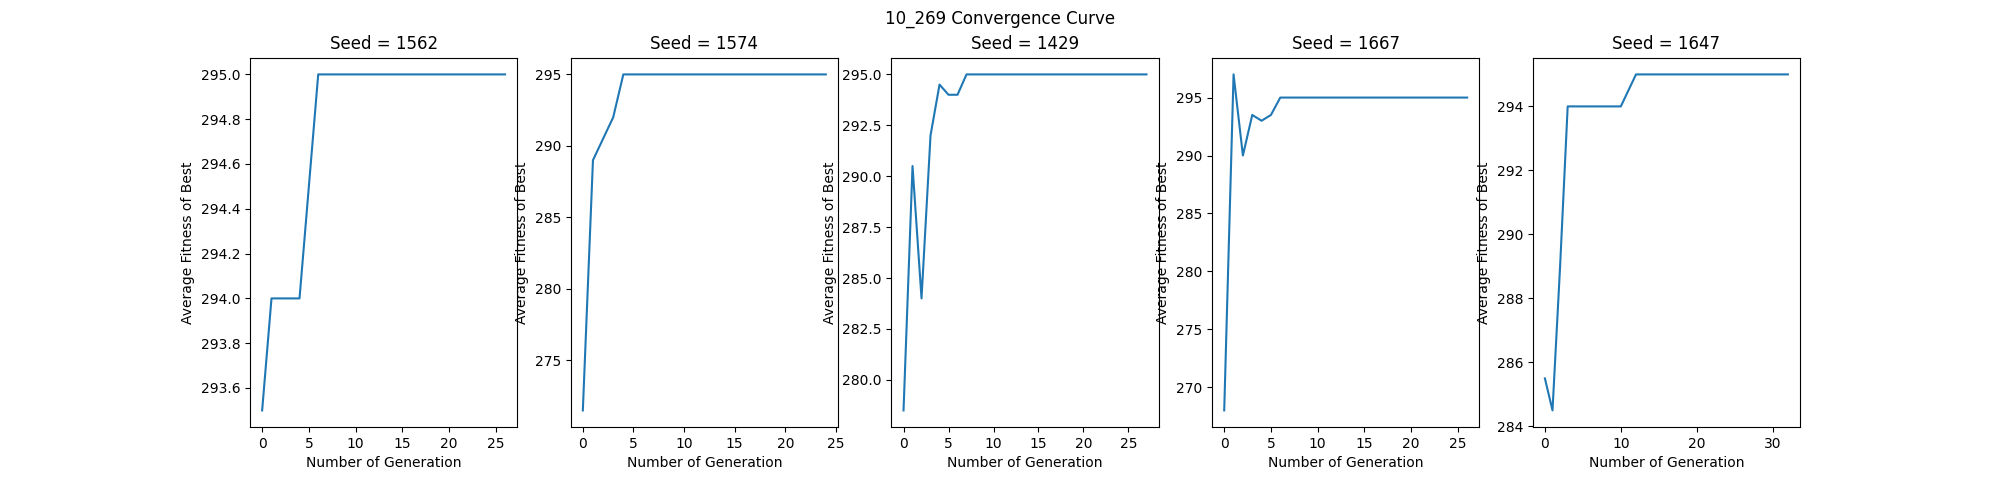
\includegraphics[width=\linewidth]{knapsack_10_269.png}
	\caption{Convergence Curve}
\end{figure}

\subsection*{23\_10000 Dataset}
\begin{center}
	\begin{tabular}{|c|c|}
		\hline
		Average Fitness of Best Average & Average Fitness of Best Standard Deviation \\
		\hline
		9766.6 & 0.7999.. \\
		\hline
	\end{tabular}
\end{center}

\begin{center}
	\begin{tabular}{|c|c|}
		\hline
		Seed & Number of iterations \\
		\hline
		1562 & 49 \\
		\hline
		1574 & 48 \\
		\hline
		1429 & 90 \\
		\hline
		1667 & 52 \\
		\hline
		1647 & 50 \\
		\hline
	\end{tabular}
\end{center}

\begin{figure}[h!]
	\centering
	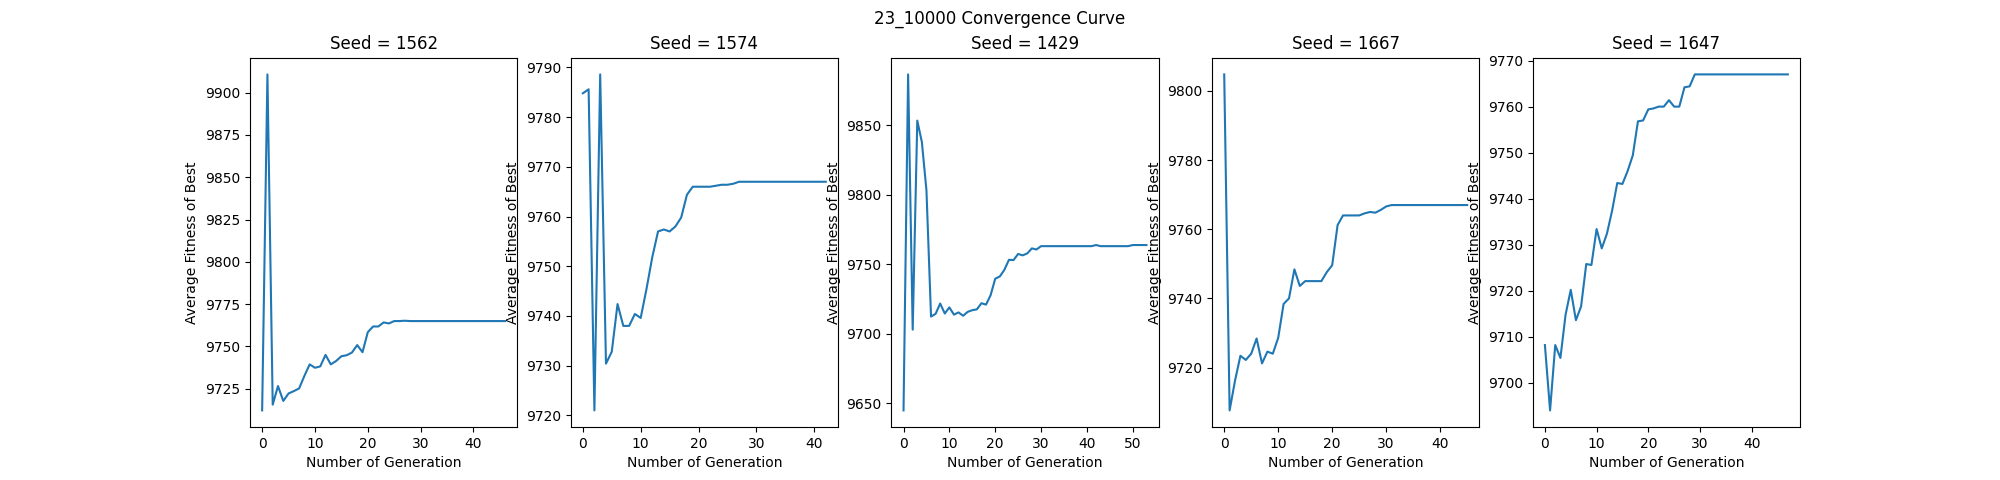
\includegraphics[width=\linewidth]{knapsack_23_10000.png}
	\caption{Convergence Curve}
\end{figure}

\subsection*{100\_995 Dataset}
\begin{center}
	\begin{tabular}{|c|c|}
		\hline
		Average Fitness of Best Average & Average Fitness of Best Standard Deviation \\
		\hline
		1435.4 & 40.9712 \\
		\hline
	\end{tabular}
\end{center}

\begin{center}
	\begin{tabular}{|c|c|}
		\hline
		Seed & Number of iterations \\
		\hline
		1562 & 65 \\
		\hline
		1574 & 58 \\
		\hline
		1429 & 50 \\
		\hline
		1667 & 55 \\
		\hline
		1647 & 64 \\
		\hline
	\end{tabular}
\end{center}

\begin{figure}[h!]
	\centering
	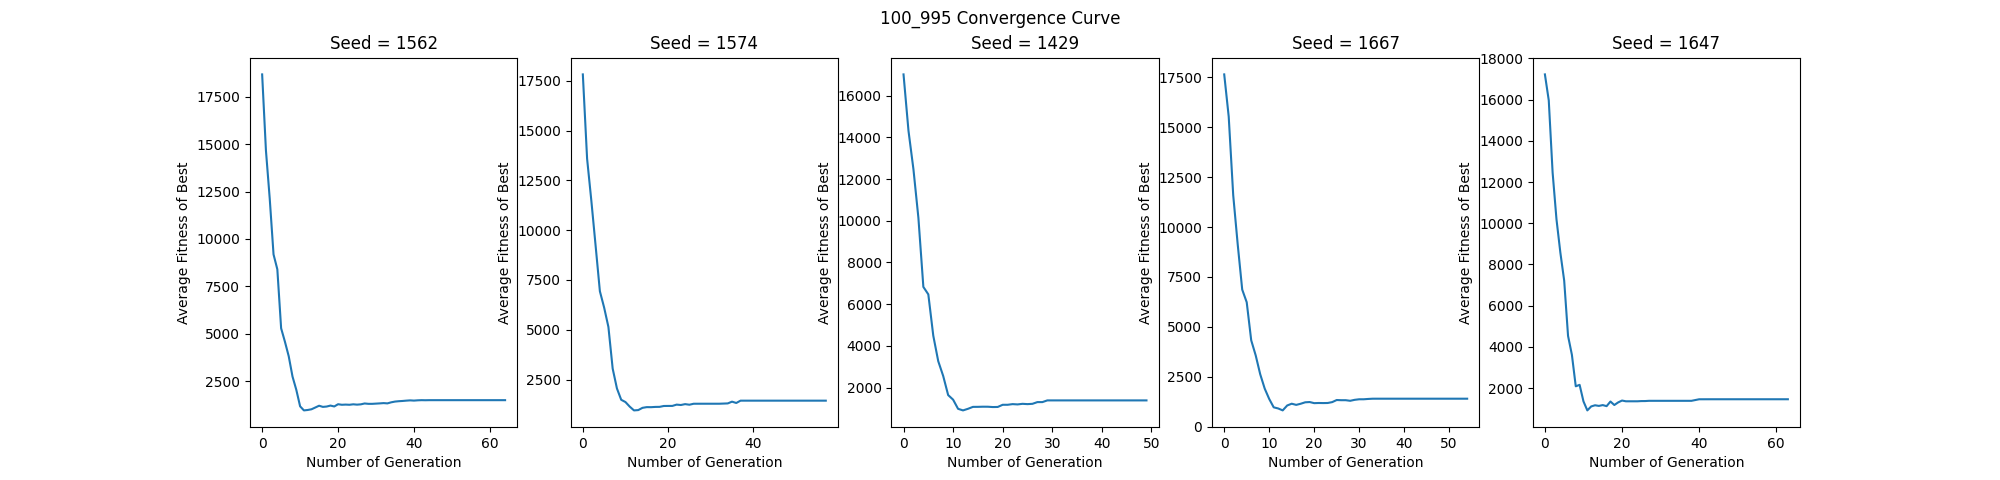
\includegraphics[width=\linewidth]{knapsack_100_995.png}
	\caption{Convergence Curve}
\end{figure}

\subsection*{Conclusion}

\section*{Part 3: Cooperative Co-evolution Genetic Programming}
\subsection*{CCGP Design}
\subsubsection*{Function and Terminal Sets}
\subsubsection*{Fitness Function and Evaluation}
\subsubsection*{CCGP Parameters}
\subsection*{Results and Discussion}

\begin{center}
	\begin{tabular}{|c|c|c|c|}
		\hline
		Seed & Best Fitness & Best Depth $f_1(x > 0)$ & Best Depth $f_2(x \le 0)$ \\
		\hline
		17 & 5.934 & 16 & 3 \\
		\hline
		35 & 5.975 & 1 & 3 \\
		\hline
		36 & 1.753 & 6 & 5 \\
		\hline
		47 & 1.589 & 1 & 17 \\
		\hline
		162 & 5.975 & 1 & 3 \\
		\hline
	\end{tabular}
\end{center}

\begin{figure}[h!]
	\centering
	\begin{subfigure}[b]{\linewidth}
		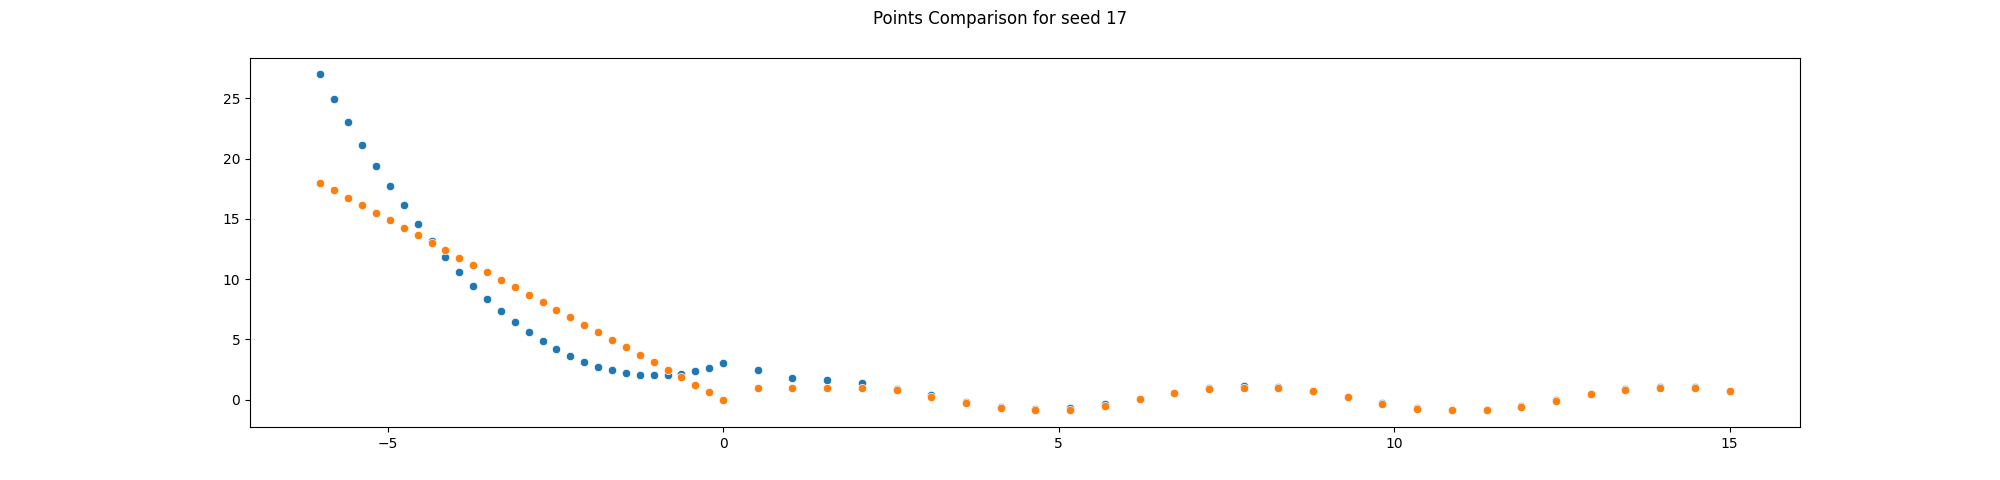
\includegraphics[width=\linewidth]{ccgp_chart_17.png}
	\end{subfigure}
\begin{subfigure}[b]{\linewidth}
	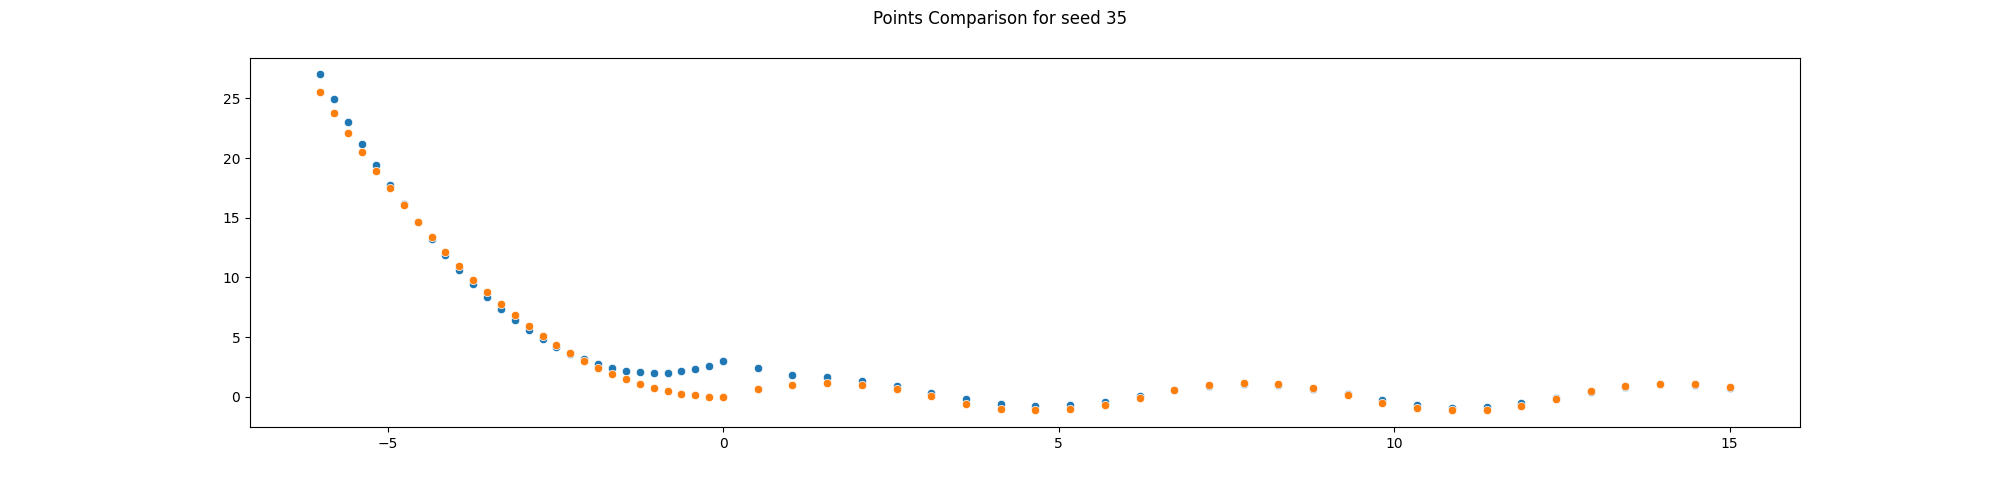
\includegraphics[width=\linewidth]{ccgp_chart_35.png}
\end{subfigure}
\begin{subfigure}[b]{\linewidth}
	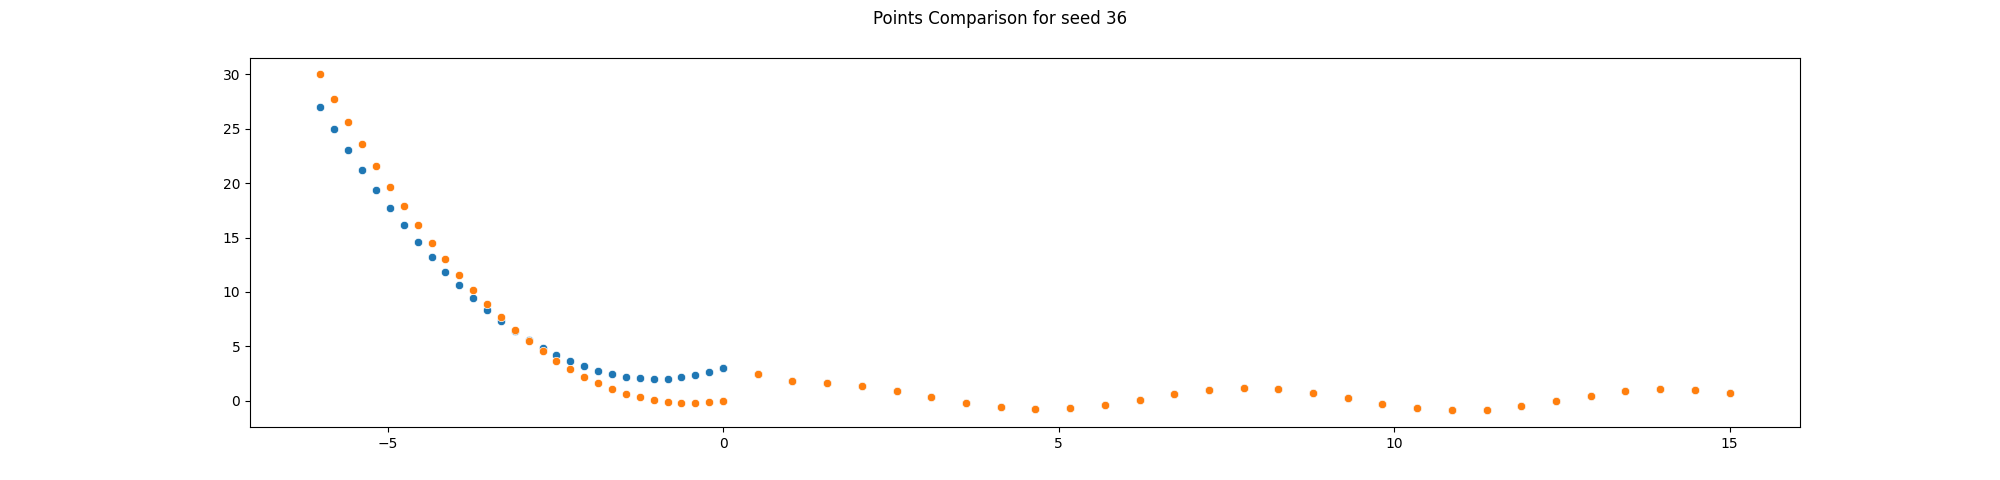
\includegraphics[width=\linewidth]{ccgp_chart_36.png}
\end{subfigure}
\begin{subfigure}[b]{\linewidth}
	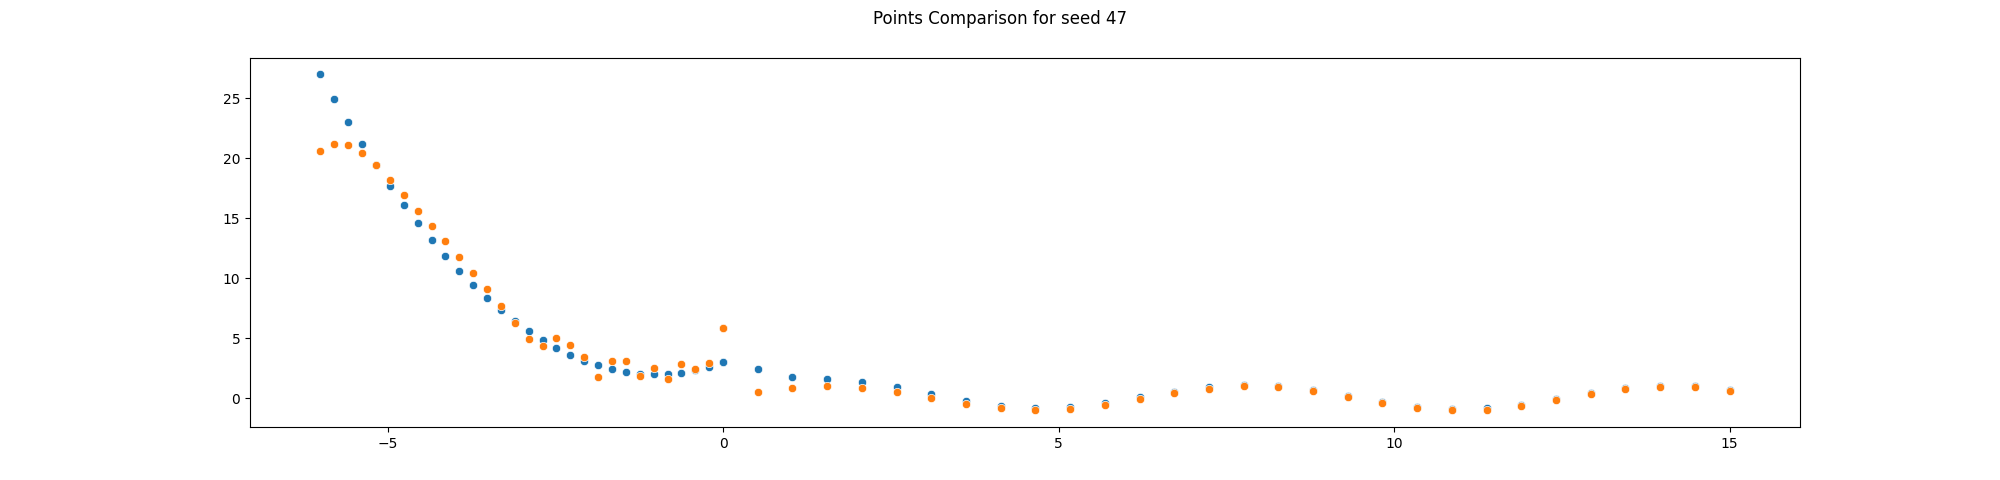
\includegraphics[width=\linewidth]{ccgp_chart_47.png}
\end{subfigure}
\begin{subfigure}[b]{\linewidth}
	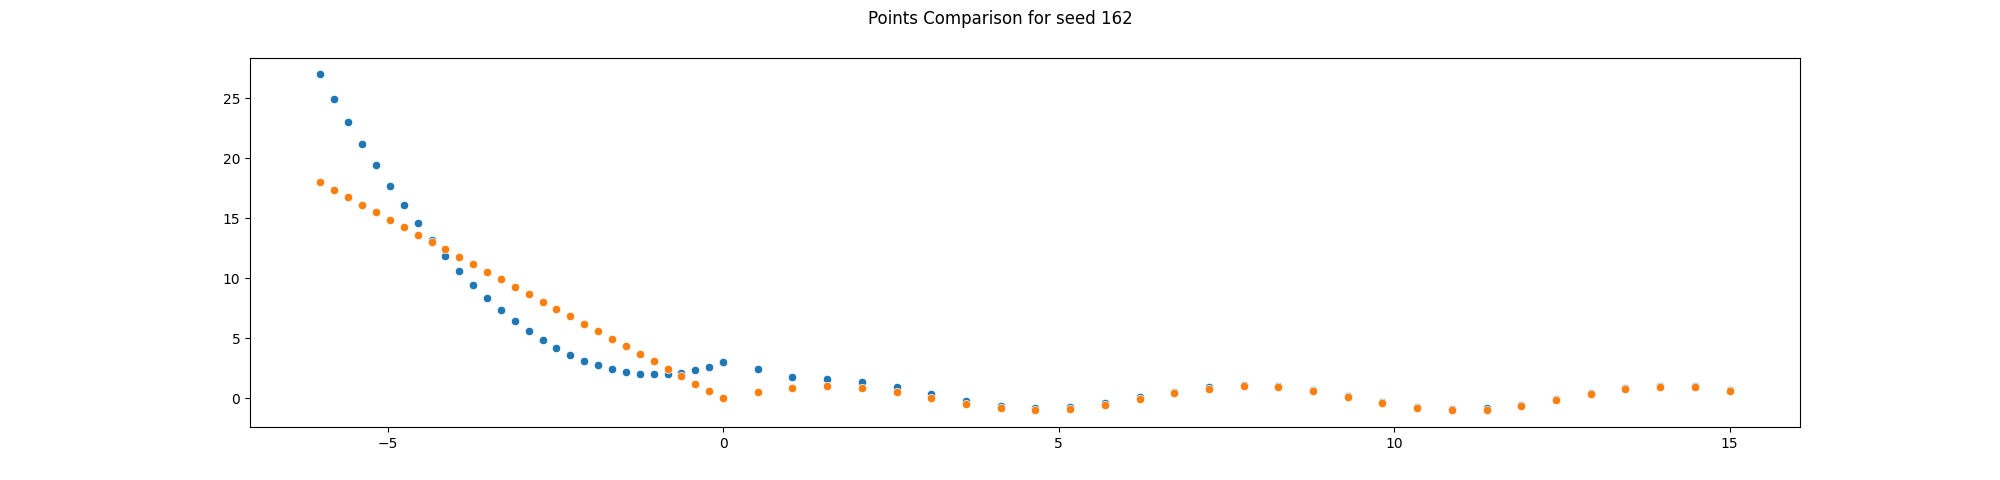
\includegraphics[width=\linewidth]{ccgp_chart_162.png}
\end{subfigure}
	\caption{Comparison of true values(blue points) and CCGP generated function values(orange points).}
\end{figure}

\begin{figure}[h!]
	\centering
	\begin{subfigure}[b]{\linewidth}
		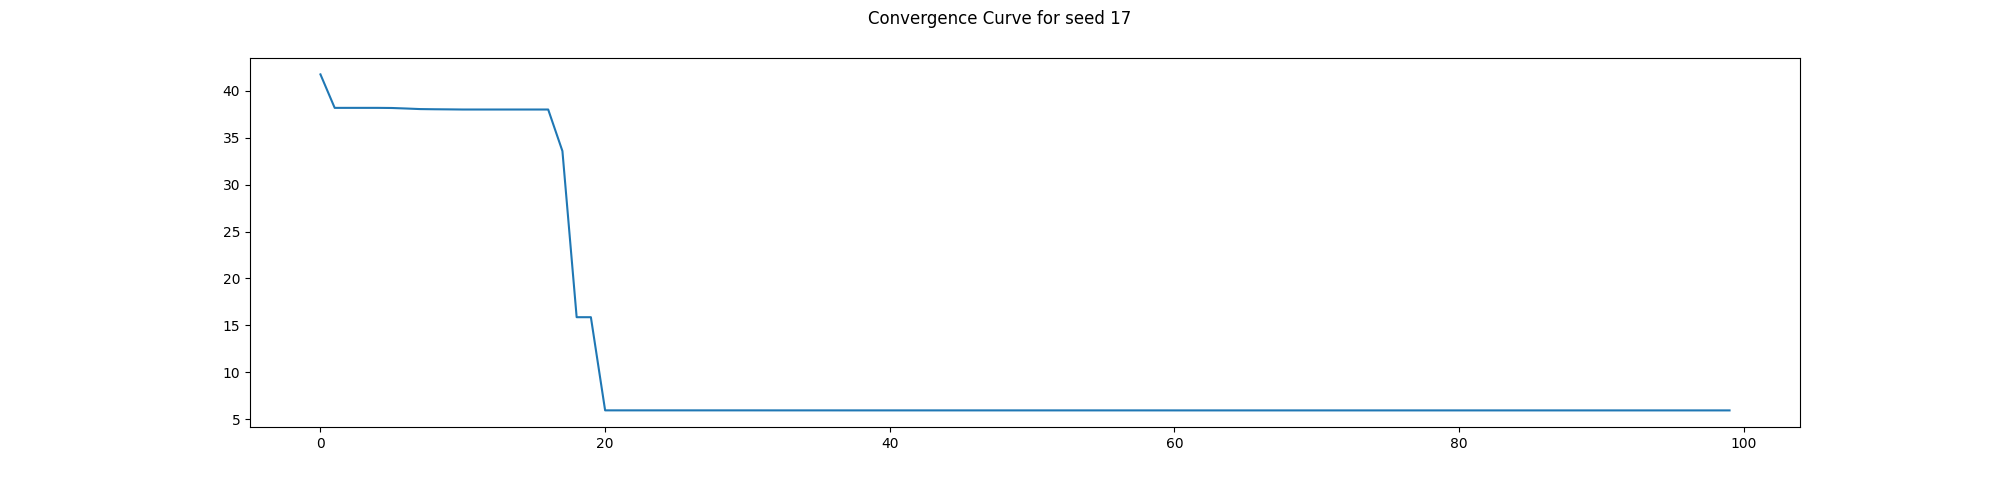
\includegraphics[width=\linewidth]{ccgp_curve_17.png}
	\end{subfigure}
	\begin{subfigure}[b]{\linewidth}
		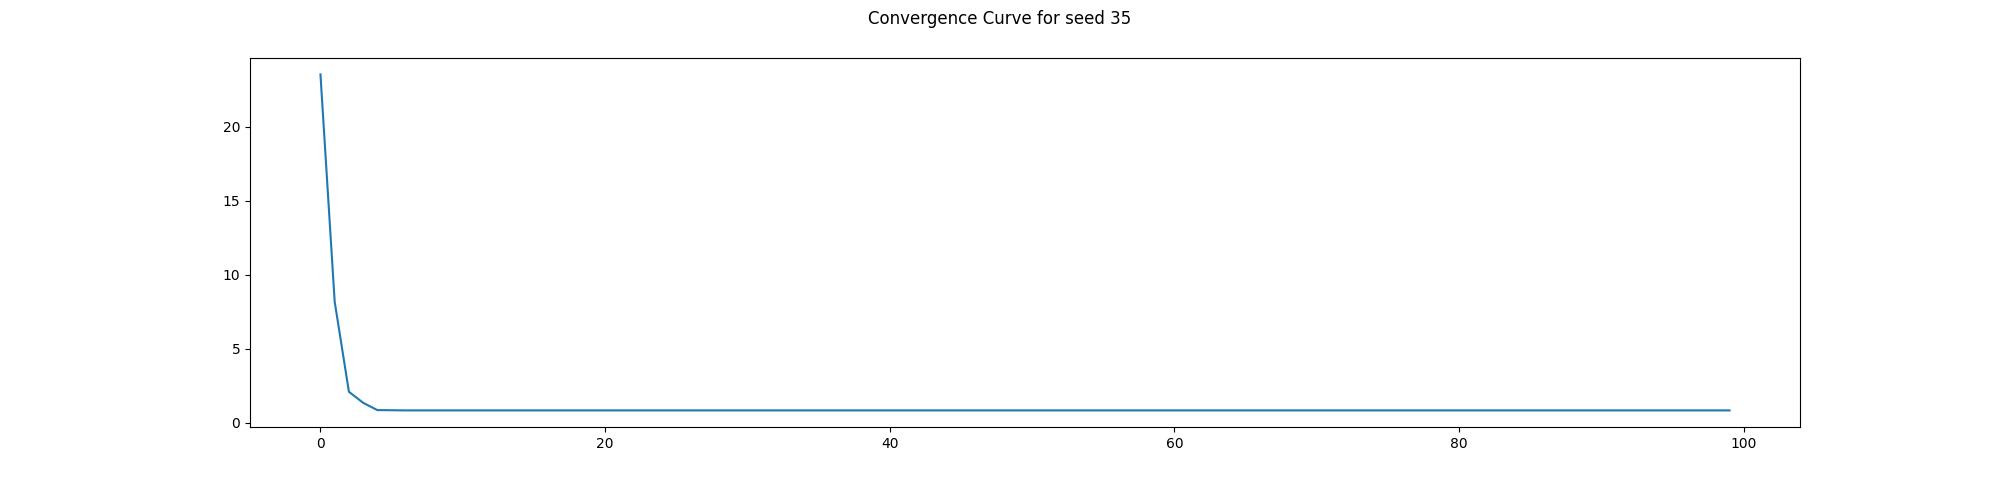
\includegraphics[width=\linewidth]{ccgp_curve_35.png}
	\end{subfigure}
	\begin{subfigure}[b]{\linewidth}
		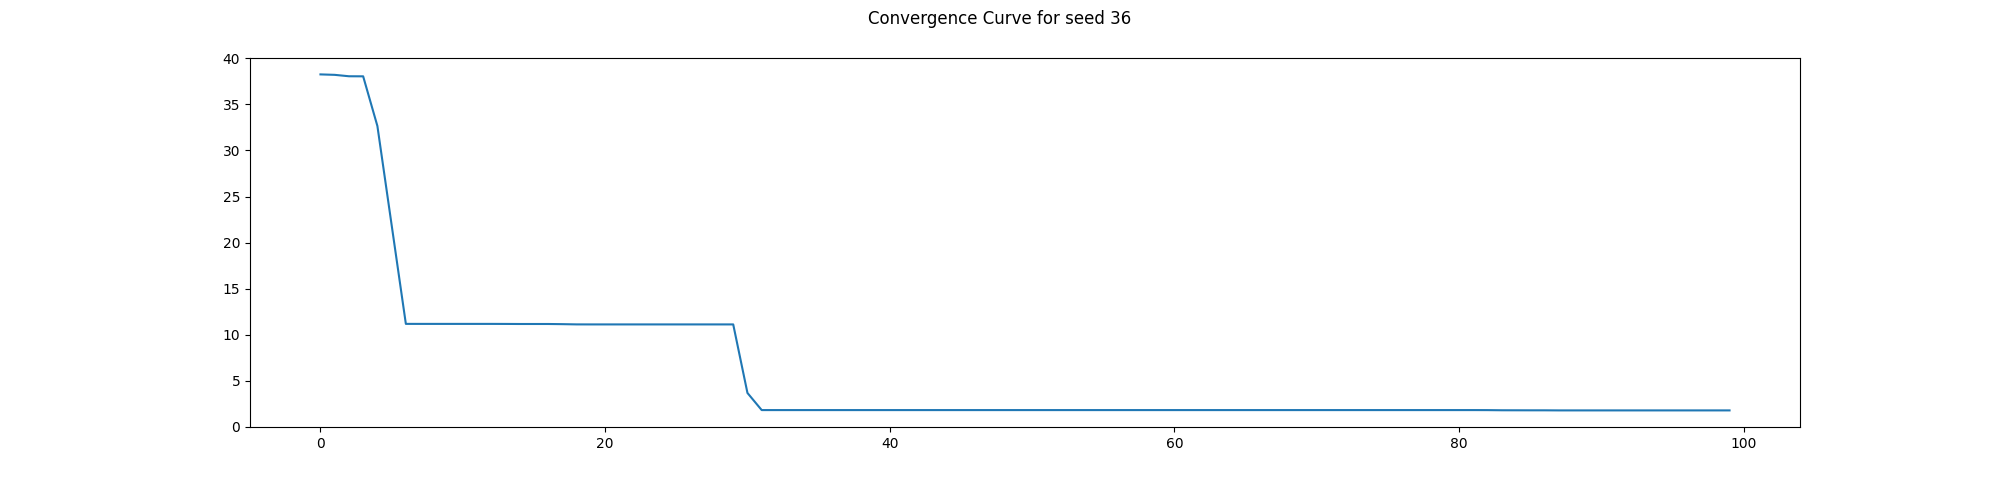
\includegraphics[width=\linewidth]{ccgp_curve_36.png}
	\end{subfigure}
	\begin{subfigure}[b]{\linewidth}
		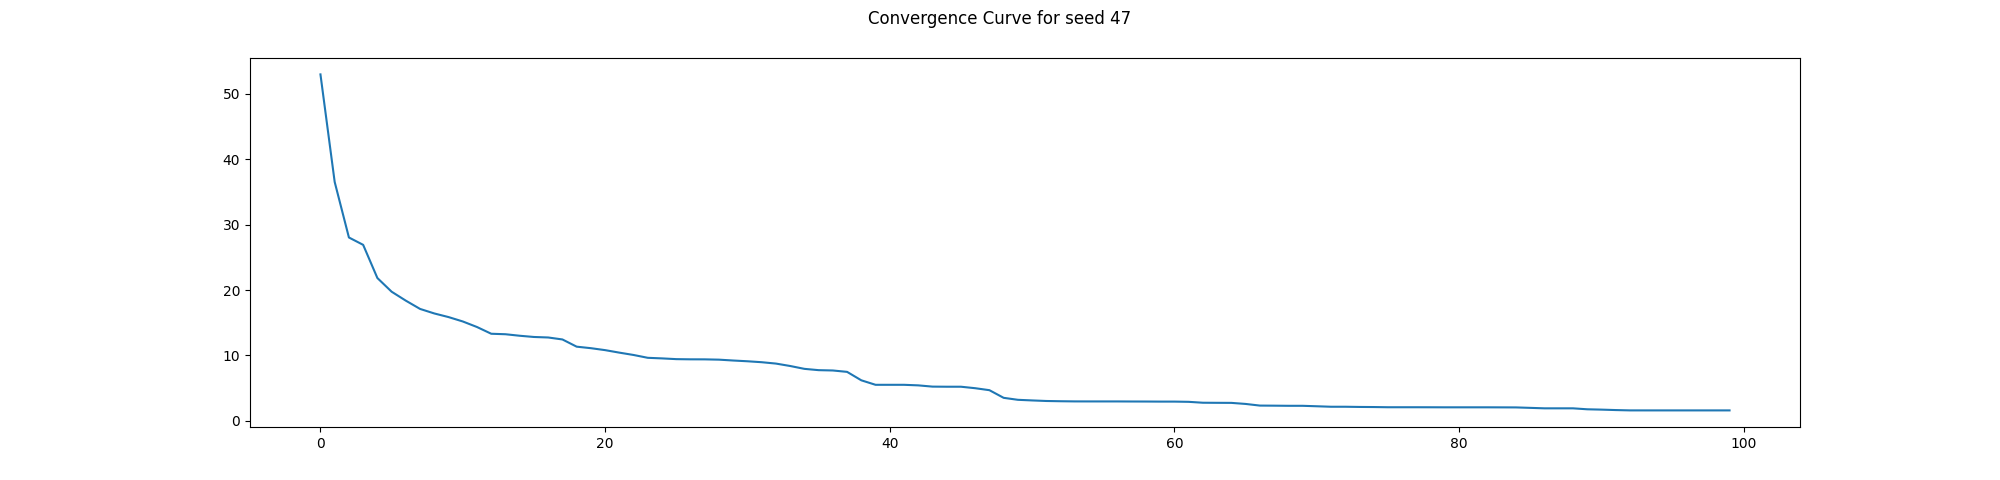
\includegraphics[width=\linewidth]{ccgp_curve_47.png}
	\end{subfigure}
	\begin{subfigure}[b]{\linewidth}
		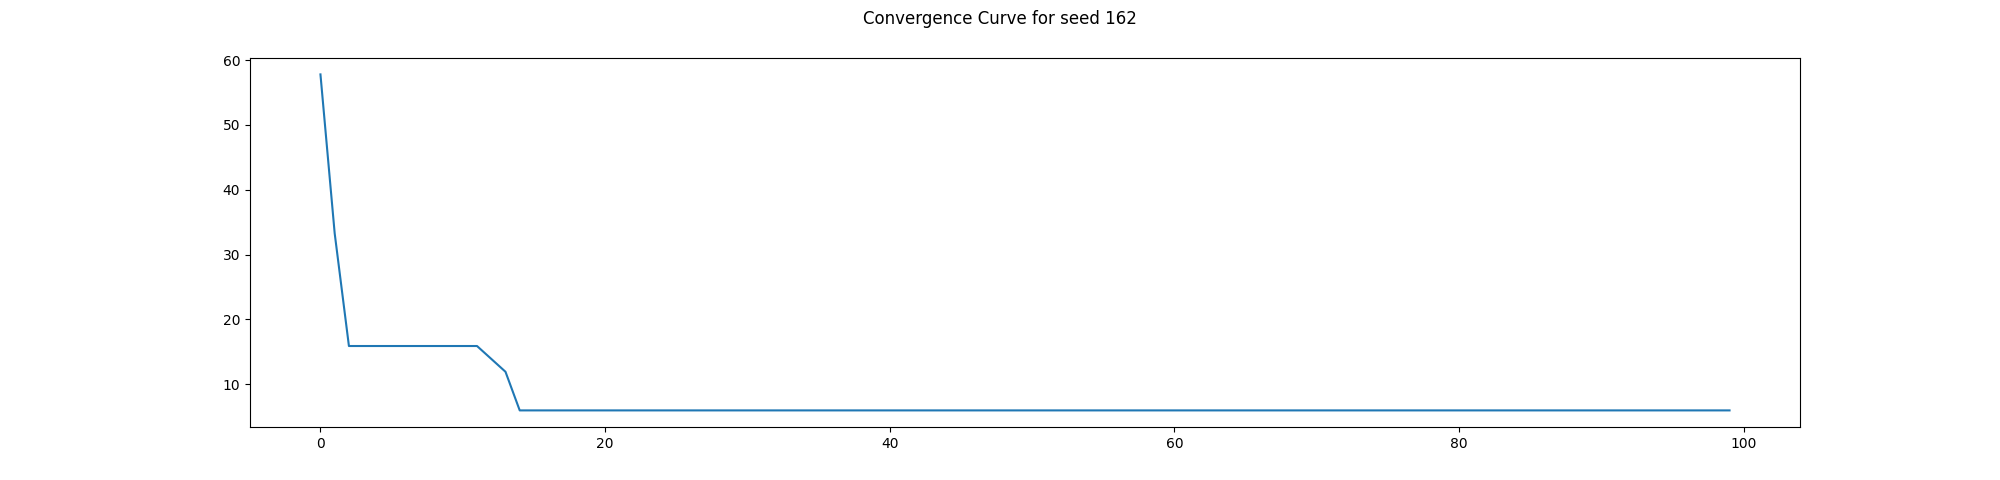
\includegraphics[width=\linewidth]{ccgp_curve_162.png}
	\end{subfigure}
	\caption{Convergence curves for each seed.}
\end{figure}

\begin{figure}[h!]
	\centering
	\begin{subfigure}[b]{\linewidth}
		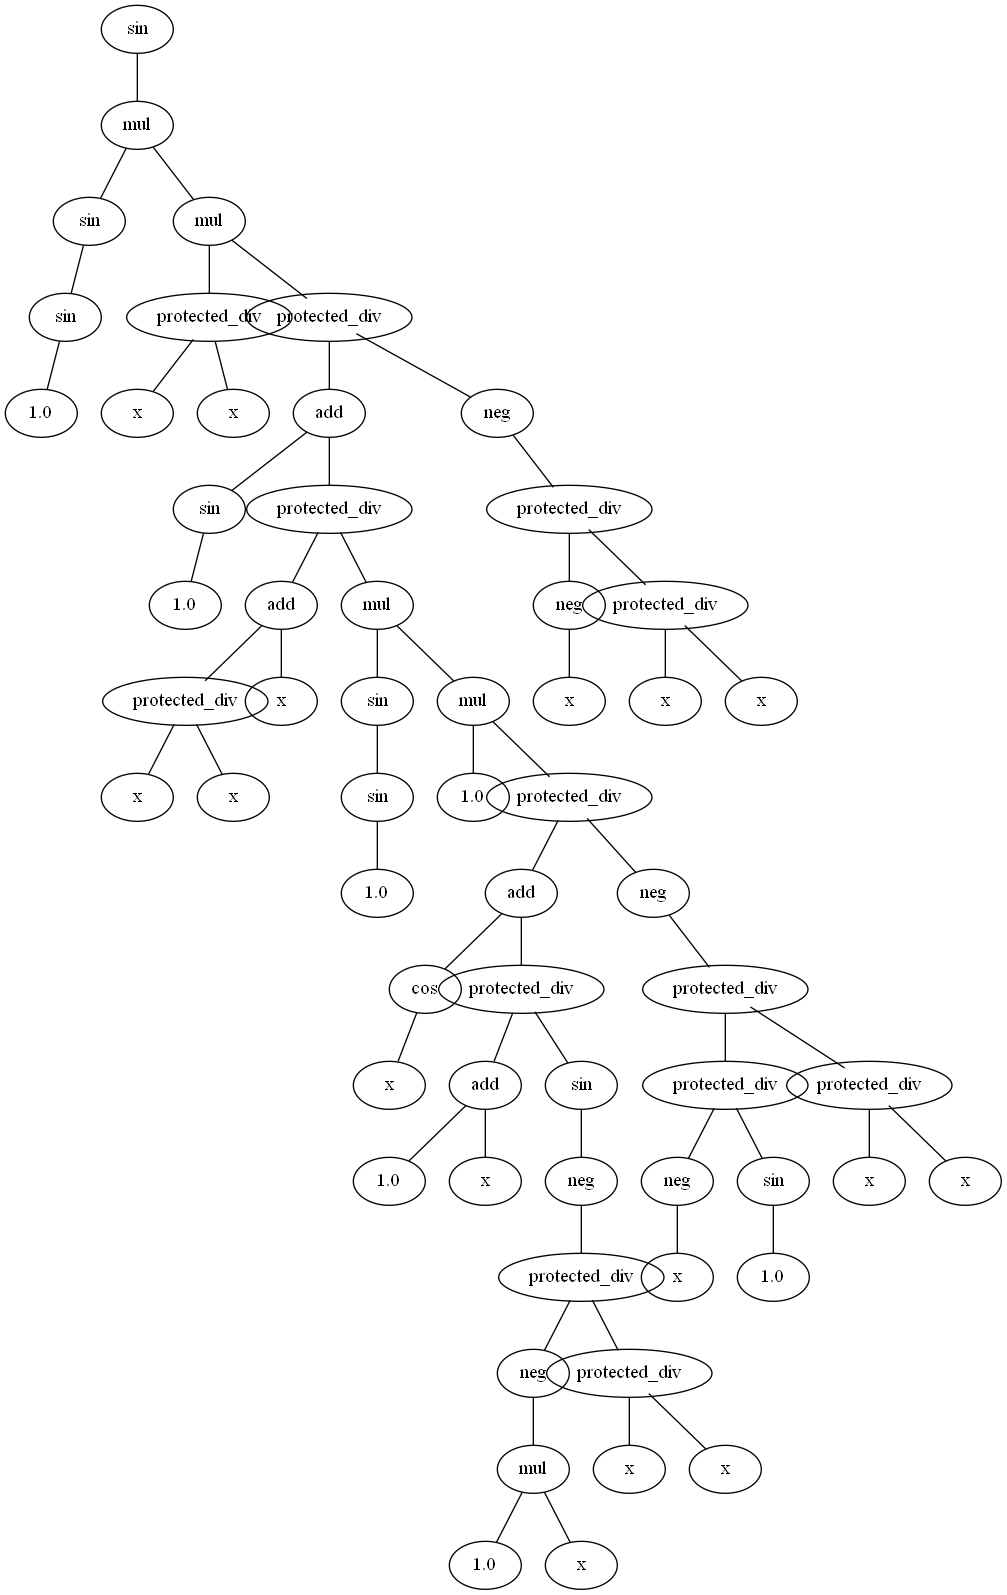
\includegraphics[width=0.5\linewidth]{ccgp_best_tree_17_1.png}
		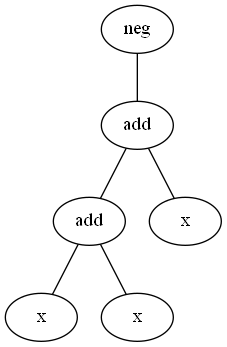
\includegraphics[width=0.5\linewidth]{ccgp_best_tree_17_2.png}
		\caption{$f_1(x > 0)$ tree(left) and $f_2(x \le 0)$ tree(right) for seed 17}
	\end{subfigure}
\end{figure}
\begin{figure}[h!]
	\centering
	\begin{subfigure}[b]{\linewidth}
		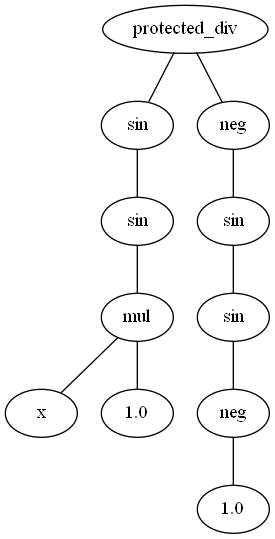
\includegraphics[width=0.5\linewidth]{ccgp_best_tree_35_1.png}
		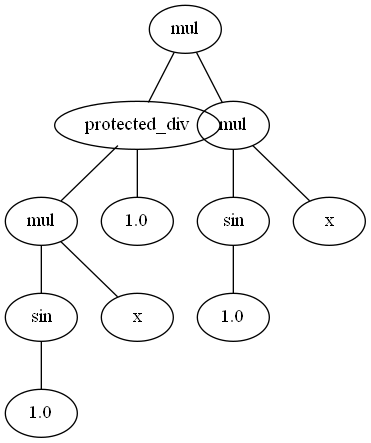
\includegraphics[width=0.5\linewidth]{ccgp_best_tree_35_2.png}
		\caption{$f_1(x > 0)$ tree(left) and $f_2(x \le 0)$ tree(right) for seed 35}
	\end{subfigure}
\end{figure}
\begin{figure}[h!]
	\centering
	\begin{subfigure}[b]{\linewidth}
		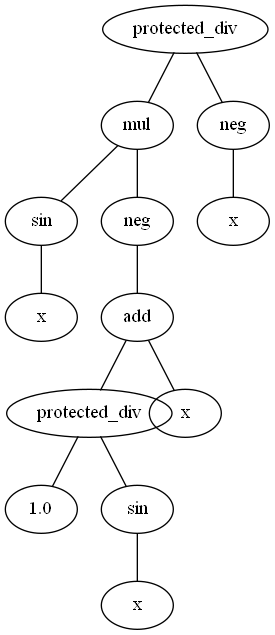
\includegraphics[width=0.5\linewidth]{ccgp_best_tree_36_1.png}
		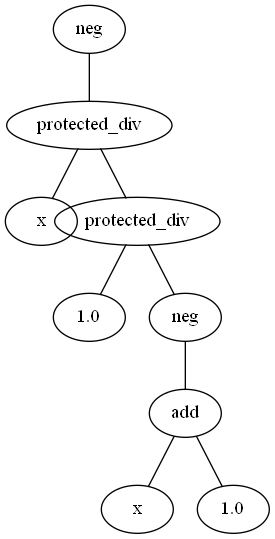
\includegraphics[width=0.5\linewidth]{ccgp_best_tree_36_2.png}
		\caption{$f_1(x > 0)$ tree(left) and $f_2(x \le 0)$ tree(right) for seed 36}
	\end{subfigure}
\end{figure}
\begin{figure}[h!]
	\centering
	\begin{subfigure}[b]{\linewidth}
		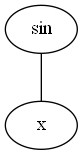
\includegraphics[width=0.1\linewidth]{ccgp_best_tree_47_1.png}
	\end{subfigure}
	\begin{subfigure}[b]{\linewidth}
		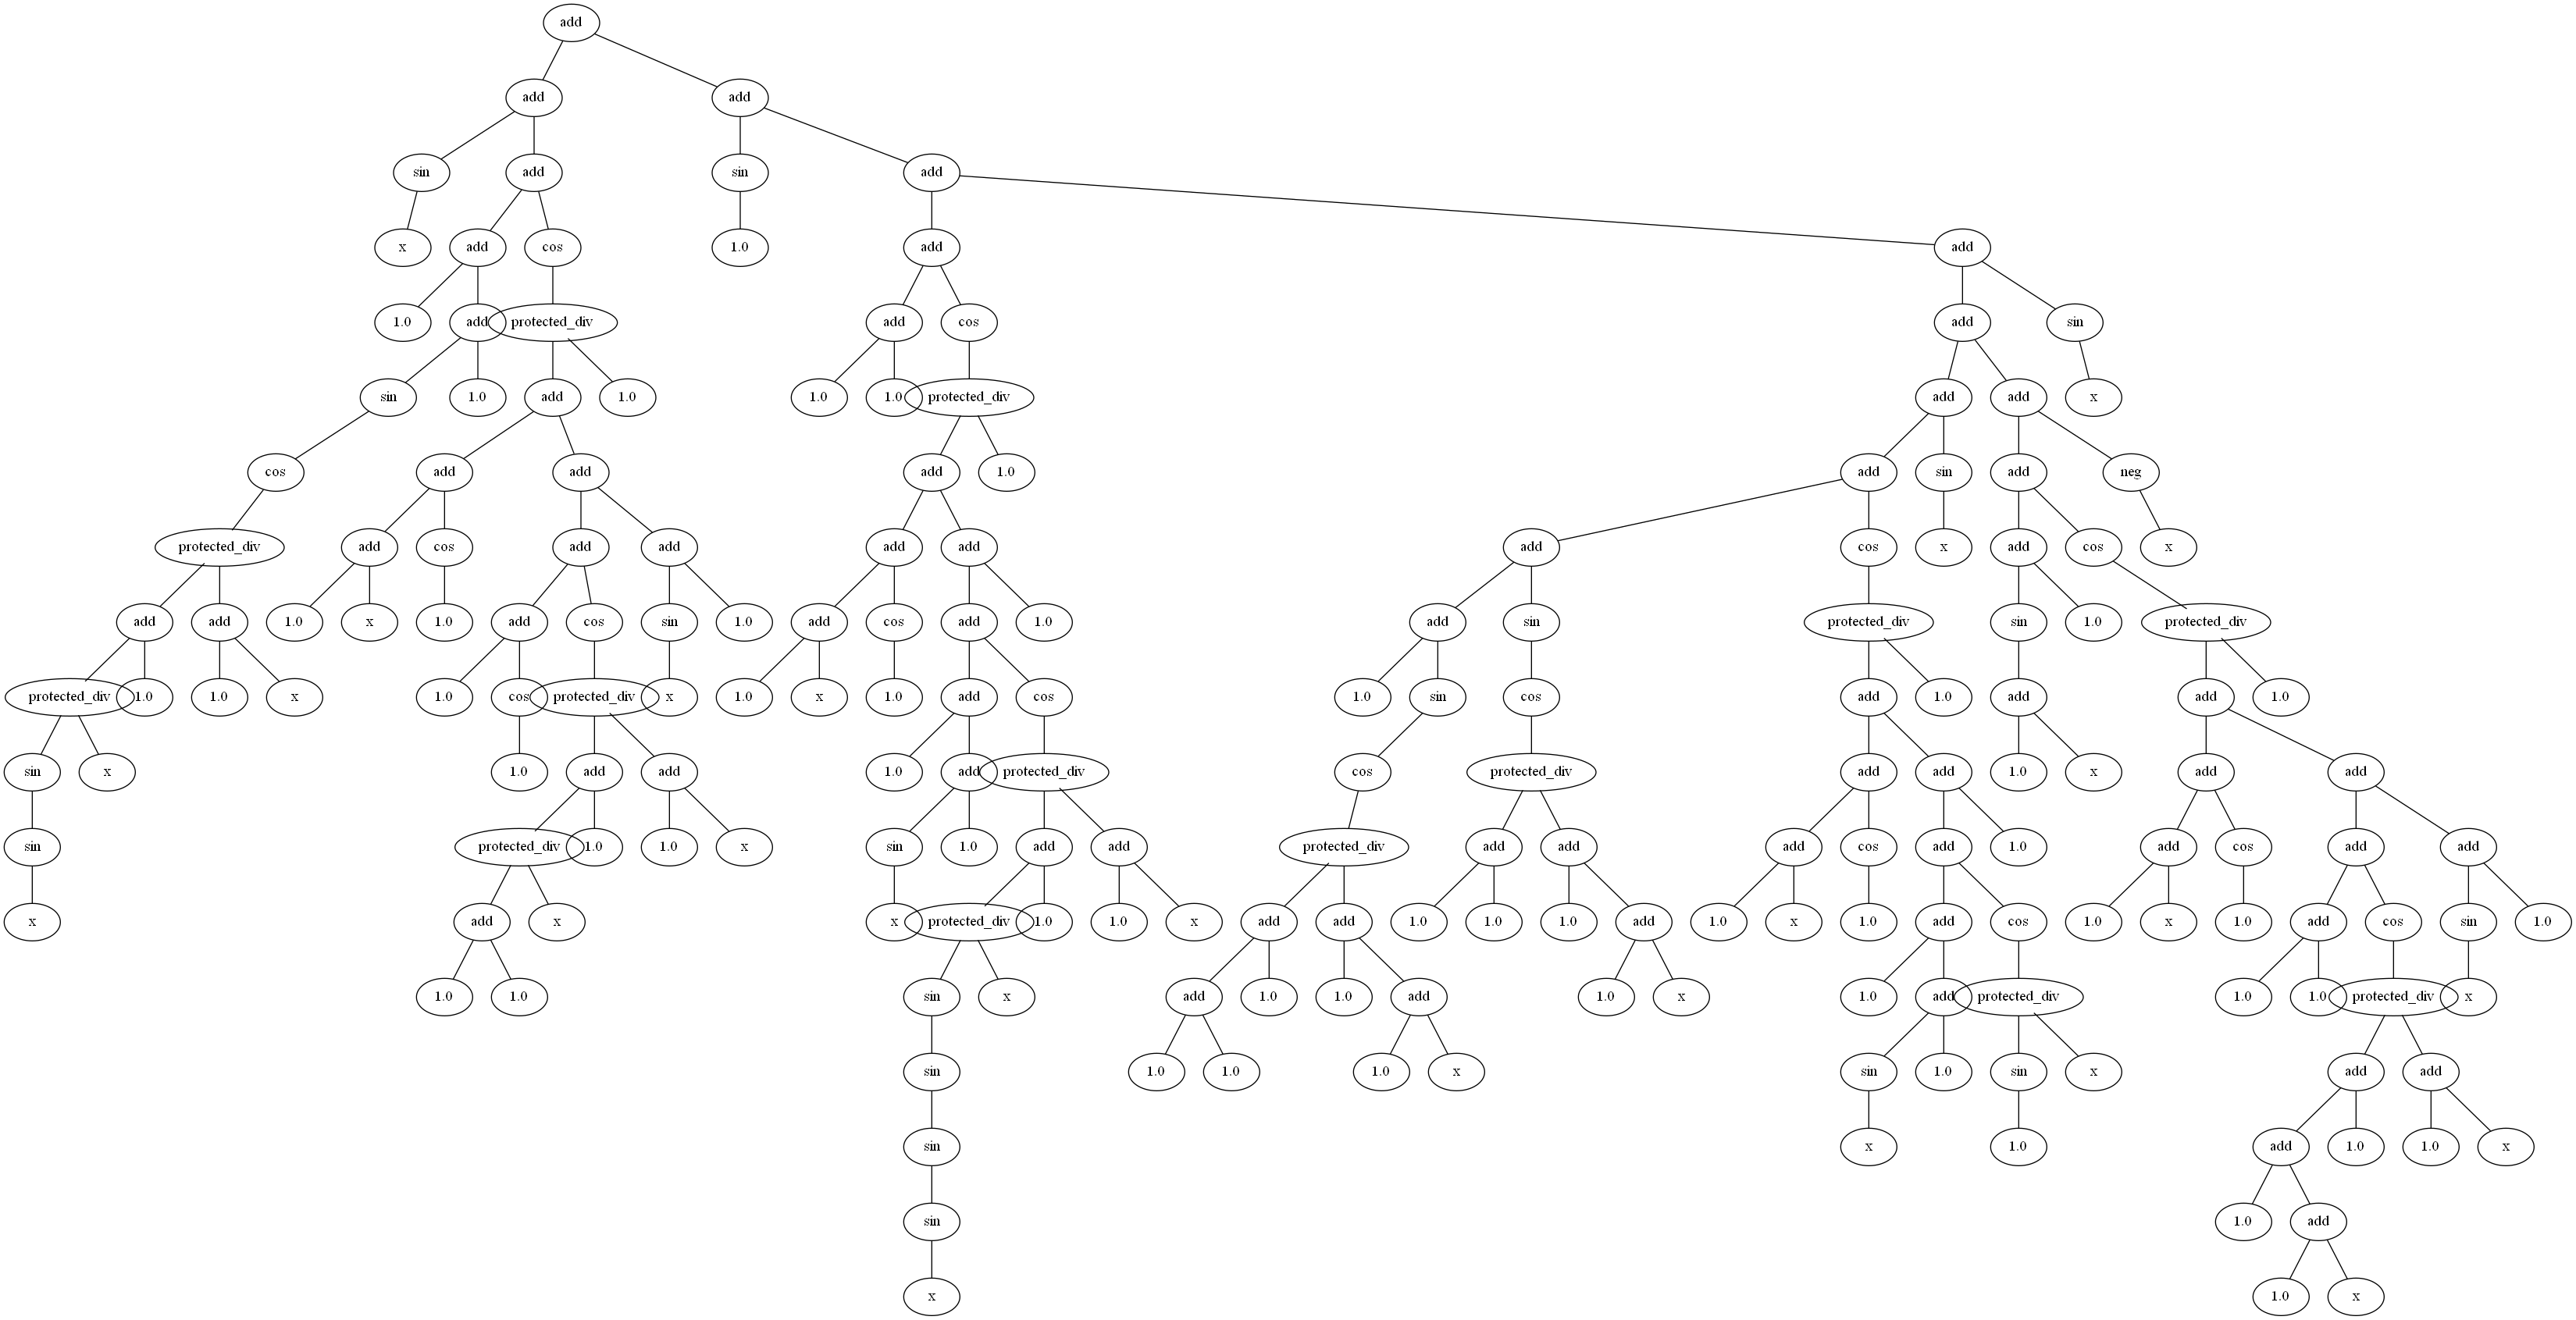
\includegraphics[width=\linewidth]{ccgp_best_tree_47_2.png}
	\end{subfigure}
	\caption{$f_1(x > 0)$ tree(top) and $f_2(x \le 0)$ tree(bottom) for seed 47}
\end{figure}
\begin{figure}[h!]
	\centering
	\begin{subfigure}[b]{\linewidth}
		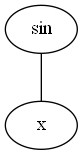
\includegraphics[width=0.5\linewidth]{ccgp_best_tree_162_1.png}
		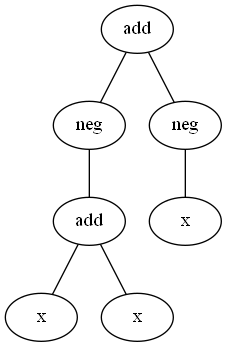
\includegraphics[width=0.5\linewidth]{ccgp_best_tree_162_2.png}
		\caption{$f_1(x > 0)$ tree(left) and $f_2(x \le 0)$ tree(right) for seed 162}
	\end{subfigure}
\end{figure}
	
\subsubsection*{Structure}
\subsubsection*{Performance}
	
\subsection*{Conclusion}

\section*{Part 4: Genetic Programming for Image Classification}
\subsection*{FLGP Trees Used}
\begin{figure}[h!]
	\centering
	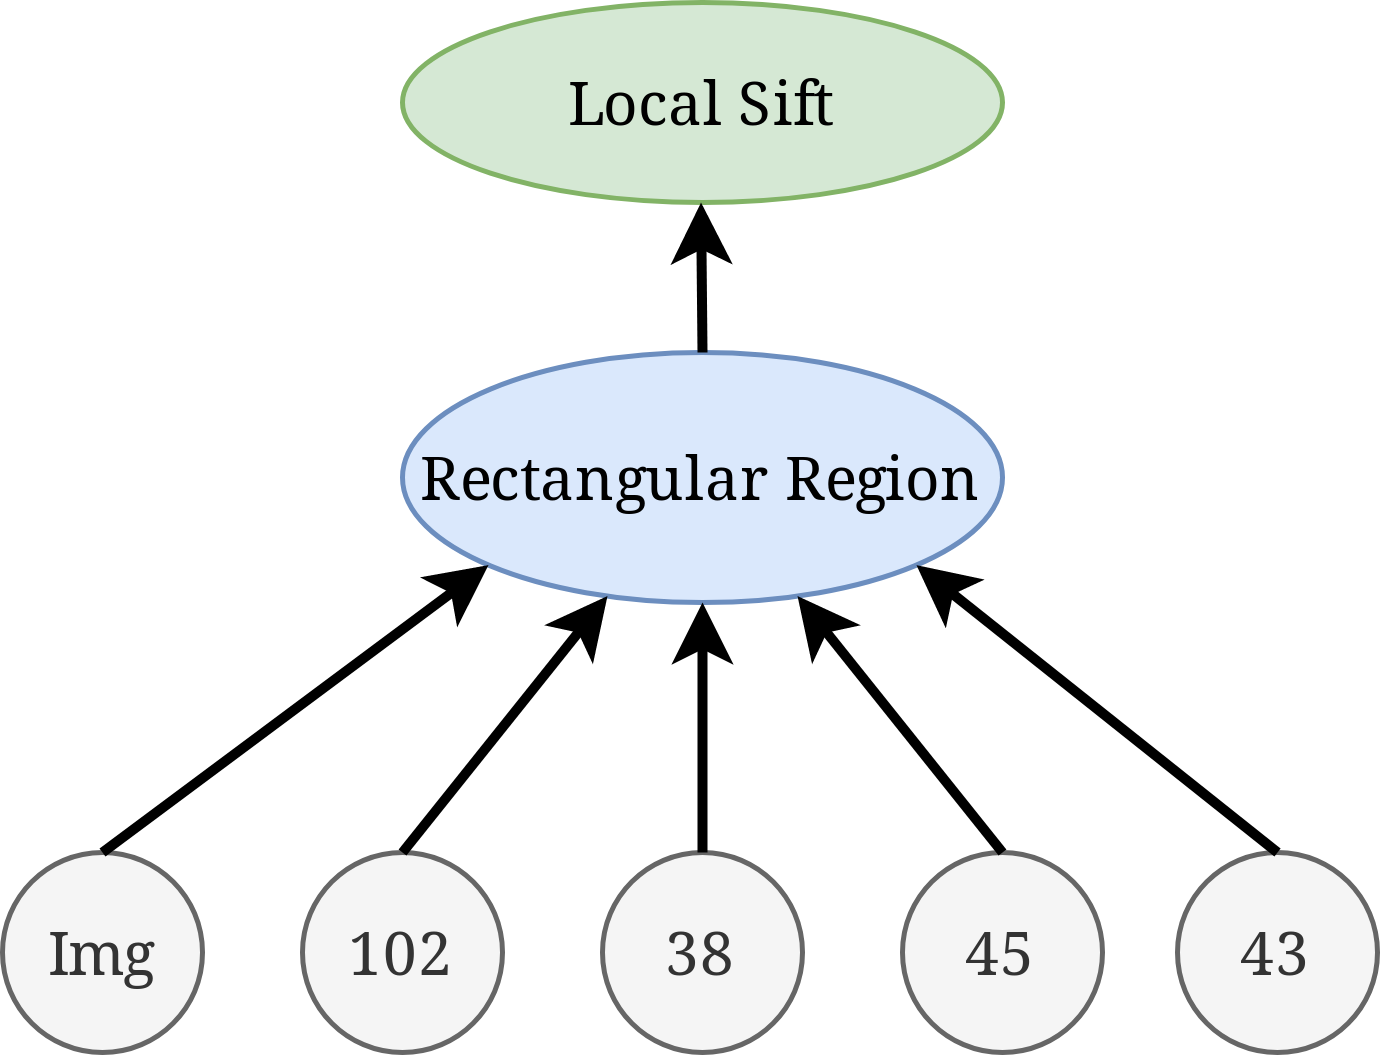
\includegraphics[width=\linewidth]{flgp_F1.png}
	\caption{Best FLGP tree for dataset FEI\_1}
\end{figure}
\begin{figure}[h!]
	\centering
	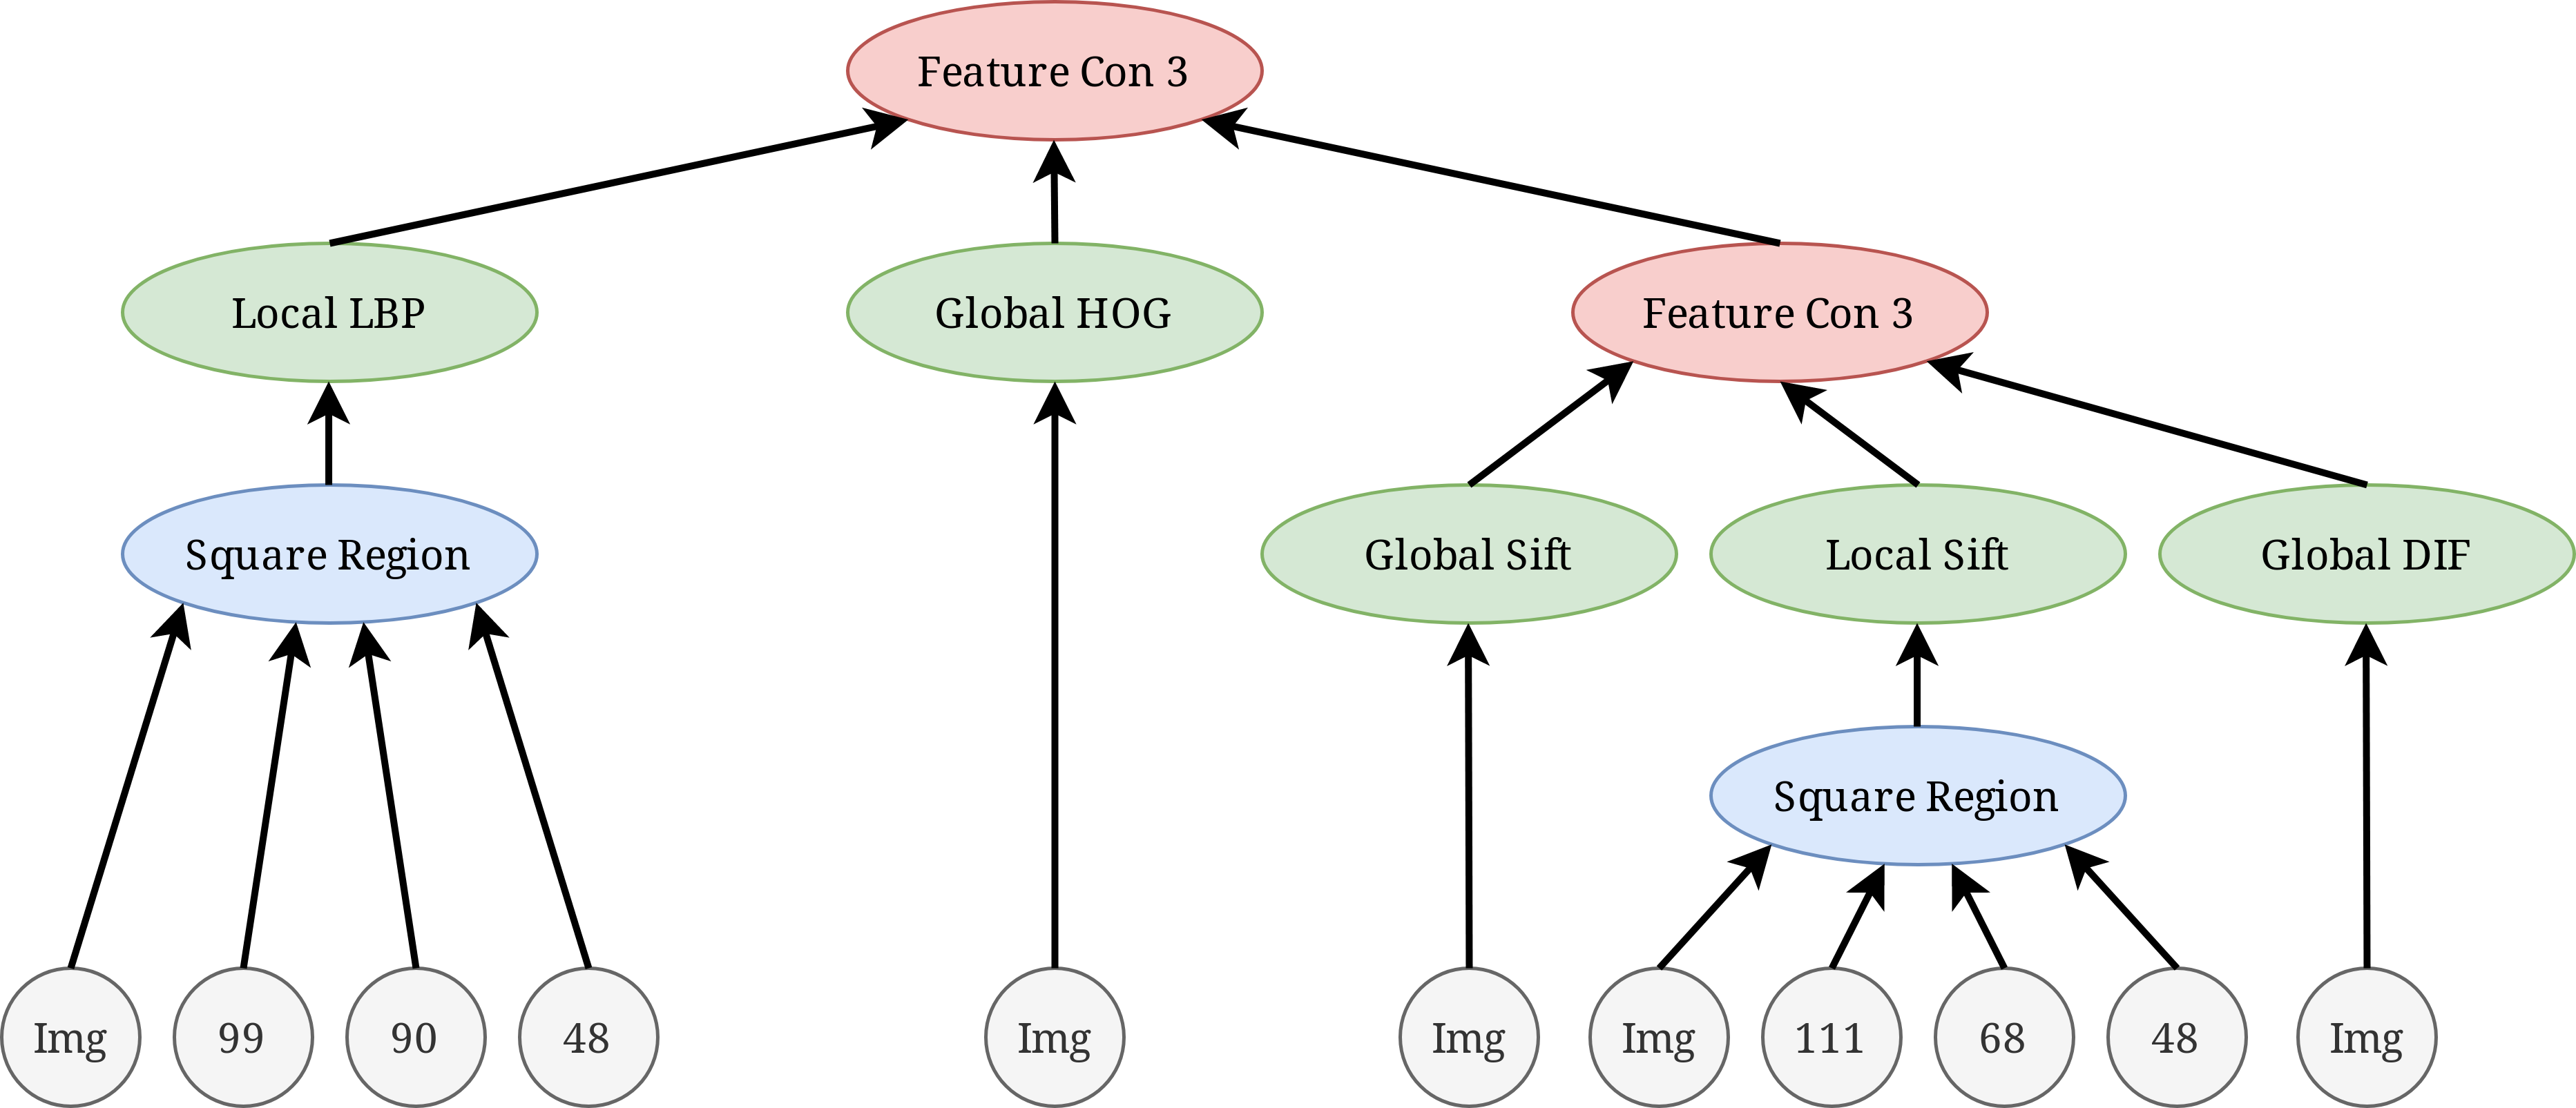
\includegraphics[width=\linewidth]{flgp_F2.png}
	\caption{Best FLGP tree for dataset FEI\_2}
\end{figure}
\begin{figure*}[h!]
	\centering
	\begin{subfigure}{0.49\linewidth}
		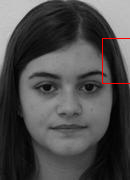
\includegraphics[width=\linewidth]{flgp_selection_f1.jpg}
		\caption{FEI\_1}
	\end{subfigure}
	\begin{subfigure}{0.49\linewidth}
		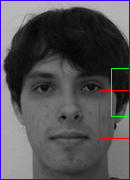
\includegraphics[width=\linewidth]{flgp_selection_f2.jpg}
		\caption{FEI\_2}
	\end{subfigure}
	\caption{Regions used by best FLGP}
\end{figure*}
\subsection*{Classifier Design and Evaluation}
\subsection*{Classifier Results and Discussion}
\clearpage
\begin{center}
	\begin{tabular}{|c|c|c|}
		\hline
		\multicolumn{3}{|c|}{FEI\_1} \\
		\hline
		Classifier & Accuracy(\%) & Training Time(seconds) \\
		\hline
		Decision Trees & 50.0 & 0.0266 \\
		\hline
		Naive Bayes & 98.0 & 0.0172 \\
		\hline
		KNN & 50.0 & 0.0168 \\		
		\hline
		\multicolumn{3}{|c|}{FEI\_2} \\
		\hline
		Classifier & Accuracy(\%) & Training Time(seconds) \\
		\hline
		Decision Trees & 88.0 & 0.0222 \\
		\hline
		Naive Bayes & 96.0 & 0.0390 \\
		\hline
		KNN & 72.0 & 0.0117 \\		
		\hline
	\end{tabular}
\end{center}
\subsection*{Conclusion}

\bibliographystyle{acm}
\bibliography{references}

\end{document}